\chapter{\ifenglish Introduction\else บทนำ\fi}

\section{\ifenglish Project rationale\else ที่มาของโครงงาน\fi}
\hspace{0.5in}
การตั้งค่าและการตรวจสอบความถูกต้องอุปกรณ์เครือข่ายในปัจจุบันนั้นสามารถทำได้ยากสำหรับบุคคลทั่วไปที่ไม่มีความเชี่ยวชาญในด้านนี้ เนื่องจากผู้ที่ต้องทำการตั้งค่าต้องมีความรู้พื้นฐานด้านชุดคำสั่งสำหรับการตั้งค่าอุปกรณ์เครือข่ายและต้องทำการตั้งค่าและตรวจสอบผ่าน Command Line Interfaces (CLIs) ซึ่งการตั้งค่าอุปกรณ์เครือข่ายในแต่ละรอบนั้นสามารถทำได้ทีละเครื่องเท่านั้น หากมีกรณีที่ผู้ดูแลระบบต้องทำการตั้งค่าอุปกรณ์หลายๆ อุปกรณ์โดยต้องใช้ชุดคำสั่งเดิมจะทำให้เกิดการทำงานที่ซ้ำซ้อนและทำให้เสียเวลาได้และในบางครั้งผู้ดูแลระบบมีโอกาสที่จะตั้งค่าอุปกรณ์เครือข่ายผิดจากการทำงานด้วยมือโดยที่ไม่ได้ตั้งใจอีกด้วย
ถึงแม้ว่าทำการตั้งค่าอุปกรณ์เครือข่ายเสร็จแล้วผู้ดูแลยังต้องทำการตรวจสอบการทำงานของอุปกรณ์เครือข่ายว่าถูกต้องหรือไม่ ซึ่งการตรวจสอบการทำงานของอุปกรณ์เครือข่ายนั้นผู้ดูแลต้องมีความรู้รวมถึงความเชี่ยวชาญในการวิเคราะห์การทำงานของอุปกรณ์เครือข่ายเนื่องจากผู้ดูแลจำเป็นต้องรู้ว่าต้องใช้ชุดคำสั่งใดในการตรวจสอบความถูกต้องและต้องรู้ว่าควรตรวจสอบข้อมูลส่วนไหนจาก output ที่ได้มา


\begin{figure}[h]
    \begin{center}
      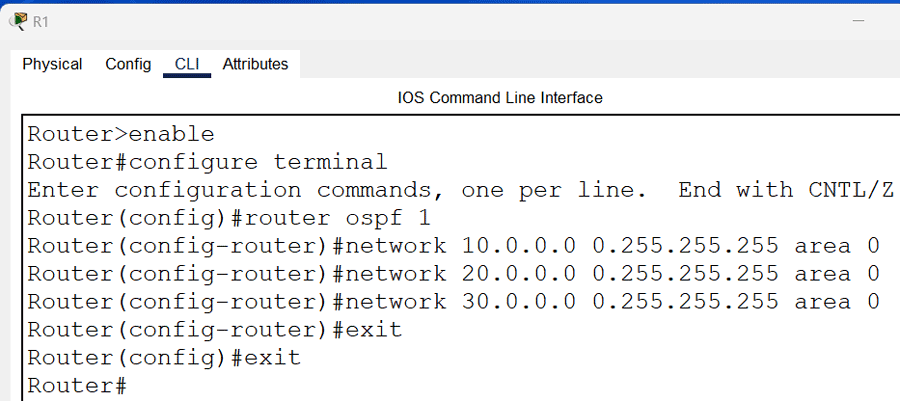
\includegraphics[scale=0.3]{RouterConf.png}
    \end{center}
    \caption[หน้าต่าง CLIs สำหรับการตั้งค่าอุปกรณ์เครือข่าย]{หน้าต่าง CLIs สำหรับการตั้งค่าอุปกรณ์เครือข่าย}
    \label{fig:RouterCLIs}
  \end{figure}

  \begin{figure}[h]
    \begin{center}
      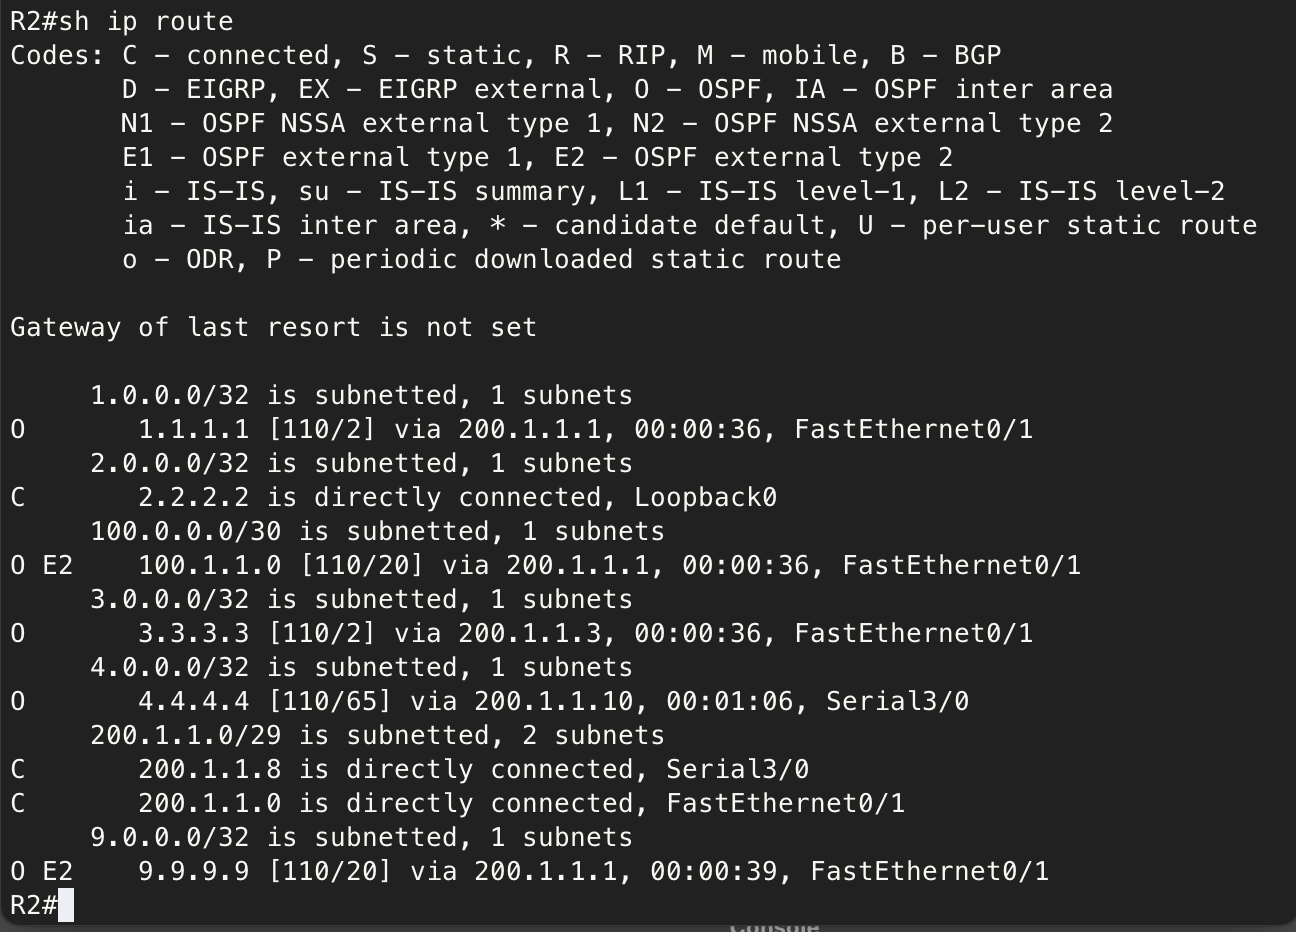
\includegraphics[scale=0.4]{shRoute.png}
    \end{center}
    \caption[หน้าต่าง CLIs ที่แสดงข้อมูล Routing Table ของ Router]{หน้าต่าง CLIs ที่แสดงข้อมูล Routing Table ของ Router}
    \label{fig:shRoute}
  \end{figure}
  \hspace{0.5in}
ในปัจจุบันมี tools สำหรับการ Automation ชื่อว่า Ansible ซึ่งเป็นเครื่องมือที่สามารถ SSH เข้าไปจัดการตั้งค่าอุปกรณ์เครือข่ายหลายๆเครื่องในครั้งเดียวได้ และมี AWX เป็น GUI สำหรับควบคุมการทำงานของ Ansible เนื่องจากการใช้งาน Ansible นั้นต้องใช้งานผ่าน CLIs ซึ่งอาจใช้งานได้ยากสำหรับผู้ใช้บางคน
ดังนั้นโครงงานนี้จึงนำ Ansible และ AWX มาประยุกต์ใช้สำหรับการตั้งค่าอุปกรณ์เครือข่าย
\section{\ifenglish Objectives\else วัตถุประสงค์ของโครงงาน\fi}
\begin{enumerate}
    \item {เพื่อเพิ่มความง่ายในการจัดการอุปกรณ์เครือข่าย}
    \item {เพื่อลดเวลาในการตั้งค่าแบะตรวจสอบอุปกรณ์เครือข่าย}
    \item {เพื่อป้องกันการผิดพลาดจากการทำงานด้วยมือ}
    \item {เพื่อพัฒนาระบบที่สามารถตั้งค่าและตรวจสอบอุปกรณ์เครือข่ายได้}
\end{enumerate}

\section{\ifenglish Project scope\else ขอบเขตของโครงงาน\fi}
\subsection{\ifenglish Hardware scope\else ขอบเขตด้านฮาร์ดแวร์\fi}
\begin{enumerate}
    \item {Router ของ Cisco}
    \item {Router ของ Huawei}
    \item {Switch ของ Cisco}
    \item {Switch ของ Huawei}
    \item {เซิฟเวอร์สำหรับใช้งาน Ansible และ AWX 1 เครื่อง (เป็นเซิฟเวอร์ที่สามารถเชื่อมต่ออินเทอร์เน็ตได้)}
\end{enumerate}
\subsection{\ifenglish Software scope\else ขอบเขตด้านซอฟต์แวร์\fi}
\begin{enumerate}
    \item {ชุดคำสั่งการตั้งค่าอุปกรณ์เครือข่ายที่ทำการกำหนดไว้}
\end{enumerate}
\section{\ifenglish Expected outcomes\else ประโยชน์ที่ได้รับ\fi}
\begin{enumerate}
    \item {ได้เรียนรู้วิธีการใช้งาน Ansible สำหรับการทำ Network Automation}
    \item {ได้ทบทวนชุดคำสั่งสำหรับการตั้งค่าอุปกรณ์เครือข่าย}
    \item {ได้เรียนรู้วิธีการตรวจสอบความถูกต้องของการทำงานอุปกรณ์เครือข่าย}
    \item {ได้เรียนรู้วิธีการสร้างและจัดการ Virtual Machine }
\end{enumerate}
\section{\ifenglish Technology and tools\else เทคโนโลยีและเครื่องมือที่ใช้\fi}
    
\subsection{\ifenglish Hardware technology\else เทคโนโลยีด้านฮาร์ดแวร์\fi}
\begin{enumerate}
    \item {อุปกรณ์เครือข่ายของ Cisco และ Huawei ซึ่งเป็นอุปกรณ์ที่รองรับคำสั่งแบบ CLIs}
\end{enumerate}
\subsection{\ifenglish Software technology\else เทคโนโลยีด้านซอฟต์แวร์\fi}
\begin{enumerate}
    \item {Ansible: เครื่องมือสำหรับทำระบบอัตโนมัติ}
    \item {AWX: เป็น GUI สำหรับให้ผู้ดูแลควบคุมการทำงานของ Ansible และใช้เป็น REST API สำหรับการคุยกับแอพพลิเคชั่นตรวจสอบ}
    \item {Python: ใช้สำหรับการพัฒนาระบบการตั้งค่าและระบบครวจสอบอุปกรณ์เครือข่าย}
\end{enumerate}
\section{\ifenglish Project plan\else แผนการดำเนินงาน\fi}

\begin{plan}{11}{2023}{2}{2024}
    \planitem{11}{2023}{11}{2023}{ศึกษาชุดคำสั่งการตั้งค่าและการตรวจสอบของ Cisco}
    \planitem{12}{2023}{1}{2024}{ศึกษาและทดลองใช้งาน Ansible}
    \planitem{1}{2024}{2}{2024}{ศึกษาและทดลองใช้งาน Ansible AWX}
    \planitem{2}{2024}{2}{2024}{design UX/UI สำหรับแอพพลิเคชั่น}
    \planitem{2}{2024}{2}{2024}{เขียนรายงาน}
\end{plan}

% Skip to 11/2024 until 3/2025
\begin{plan}{11}{2024}{3}{2025}
    \planitem{11}{2024}{12}{2024}{สร้างระบบการตั้งค่าอุปกรณ์เครือข่าย}
    \planitem{11}{2024}{1}{2025}{สร้างระบบตรวจสอบความถูกต้องของอุปกรณ์เครือข่ายภายในแอพพลิเคชั่น}
    \planitem{11}{2024}{1}{2025}{สร้าง UI สำหรับแอพพลิเคชั่น}
    \planitem{1}{2025}{2}{2025}{แก้ไขรูปแบบการแสดงผล output ของ AWX}
    \planitem{2}{2025}{3}{2025}{ทดสอบและแก้ไขความถูกต้องของการทำงานของระบบ}
    \planitem{3}{2025}{3}{2025}{เขียนรายงานและส่ง Final Project}
\end{plan}

\section{\ifenglish Roles and responsibilities\else บทบาทและความรับผิดชอบ\fi}
\begin{itemize}
    \item นาย ชลนันต์ ทองไทย รับผิดชอบในส่วนการพัฒนาระบบแอพพลิเคชั่นตรวจสอบความถูกต้องอุปกรณ์เครือข่าย
    \item นาย นายทัตพงศ์ เสริมสุข รับผิดชอบในส่วนการพัฒนา UI ของแอพพลิเคชั่นตรวจสอบ
    \item นายศุภณัฐ วังทิพย์ รับผิดชอบในส่วนการทำงานของ Ansible และ AWX
\end{itemize}

\section{\ifenglish%
Impacts of this project on society, health, safety, legal, and cultural issues
\else%
ผลกระทบด้านสังคม สุขภาพ ความปลอดภัย กฎหมาย และวัฒนธรรม
\fi}

\hspace{0.5in}
ผู้จัดทำมองว่าโครงงานนี้จะสามารถช่วยให้ผู้ที่ยังไม่มีความชำนาญในชุดคำสั่งการตั้งค่าอุปกรณ์เครือข่ายของ Cisco/Huawei มีความสามารถในการ ตั้งค่า ตรวจสอบ อุปกรณ์เครือข่ายได้โดยที่มีความเชี่ยวชาญที่ไม่มากและใช้เวลาในการทำกระบวนการดังกล่าวน้อยลง ทำให้สามารถมีเวลาในการทำกิจกรรมอย่างอื่นหรือสามารถพักผ่อนได้มากขึ้นกว่าเดิม
